\documentclass{beamer}
\usepackage[latin1]{inputenc}
\usepackage{latexsym}

\usepackage{listings}
\lstset{language=XML,showspaces=false,showtabs=false}

\usepackage[german]{babel}

\usetheme{Berlin}
\mode<presentation>

\newcommand{\includepng}[1]{\includegraphics[bb=-100 0 200 475, scale=0.35]{#1}}


\title{Adaptive Informationsverbreitung mittels RSS und Publish/Subscribe}
\author{Friedemann Zintel}
\date{18. Januar 2007}

\begin{document}
\bibliographystyle{ieeetr}

\begin{frame}

  \titlepage

\end{frame}

\section*{Outline}
\begin{frame}

  \tableofcontents
  
\end{frame}

\section{Einleitung}

\begin{frame}
  
  RSS: Really-Simple-Syndication
  \vspace{0.5cm}
  \begin{itemize}
  \item Standard zur Verbreitung von Informationen im Internet
  \item Dateiformat ist XML-basiert
  \item RSS-Feed ist einem Channel zugeordnet
  \item Verbreitung mittels Pull
  \item Beispiele: Nachrichten-Schlagzeilen, Blogs, Podcasting (anbieten von Medien-Dateien, z.B. mp3)
  \end{itemize}
  
\end{frame}

\section{Motivation}
\begin{frame}
  
  \frametitle{Anwendersicht: Was man gerne h�tte ...}
  \begin{itemize}
  \item Automatische Benachrichtigung �ber Feed-Aktualisierungen
  \item Aktualit�t der Feeds
  \item Definition von komplexeren Filtern: zur \dots
    \begin{list}{}{}
    \item \dots individuellen Vorselektion der Feeds
    \item \dots anbieter�bergreifenden Auswahl von Feeds
    \end{list}
  \end{itemize}
  
\end{frame}

\begin{frame}
  
  \frametitle{Stand der Dinge}
  \begin{itemize}
  \item RSS: Kein push-basiertes Pub/Sub $\rightarrow$ Client/Server
  \item Feeds m�ssen von Anwendersoftware heruntergeladen werden (Polling)
  \item Vordefinierte Channel $\rightarrow$ thematische Zuordnung auf RSS-Server-Seite
  \item Definition von Filtern nur auf Anwenderseite m�glich
  \end{itemize}
  
  \pause
  Probleme:
  \begin{itemize}
  \item Polling:
    \begin{list}{$\longrightarrow$}{}
    \item Gro�er Datenverkehr im Netz
    \item Hohe Server-seitige Last
    \end{list}
  \item Filterdefinition nur beim Anwender:
    \begin{list}{$\longrightarrow$}{}
    \item Alle Feeds m�ssen heruntergeladen werden
    \end{list}
  \end{itemize}
  \nocite{Hicks:2004:RSSBandwith}
  
\end{frame}

\begin{frame}
  
  \frametitle{Ziel}
  \begin{itemize}
  \item \glqq Entlastung\grqq der RSS-Server
  \item Reduzierung des Datenverkehrs aufgrund von Polling
  \item Erh�hung des Aktualit�tsgrades der Feeds auf Nutzerseite
  \item Erm�glichung der Subscriber-seitigen Definition von Filtern
  \end{itemize}
  
\end{frame}

\section{Verwandte Arbeiten}
\subsection*{FeedTree}

\begin{frame}
  \frametitle{FeedTree \cite{SandlerEtAl:2005:FeedTree}}
  \begin{itemize}
  \item Basiert auf Scribe \cite{SCRIBE}
  \item Signierte RSS-Dokumente werden per Multicast an alle Subscriber gesendet, die dieses abonniert haben
  \item Abonnement erfolgt durch Beitritt zu einer Gruppe
  \item Thema einer Gruppe entspricht der ID des angebotenen RSS-Feeds (URL)
  \end{itemize}
\end{frame}

\begin{frame}
  Vorteile:
  \begin{itemize}
  \item Zeitnahe Benachrichtgung �ber Feed-Aktualisierungen m�glich
  \item Bandbreiten werden gespart
  \item Authentizit�tspr�fung durch Signierung
  \item Wiederbeschaffung von Feeds durch Zwischenspeicherung in Caches
  \end{itemize}
  \pause
  \vspace{0.5cm}
  Nachteile:
  \begin{itemize}
  \item Zus�tzliche Software auf Anbieterseite erforderlich
  \item keine erweiterten Filtertechniken m�glich
  \item Nur ein Publisher vorhanden $\longrightarrow$ wirkt sich nachteilig auf Aktualit�tsgrad aus
  \end{itemize}
\end{frame}  

\subsection*{CMS-ToPSS}

\begin{frame}
  \frametitle{CMS-ToPSS \cite{PetrovicEtAl:2005:CMS-ToPSS}}
  \begin{itemize}
  \item Erweiterung zu Content-Management-Systemen
  \item Nutzt Notifikationssystem G-ToPSS: inhaltsbasierte Filterung durch GQL
  \end{itemize}
\end{frame}

\begin{frame}
  Vorteile:
  \begin{itemize}
  \item Flexible und m�chtige Filterdefinitionen sind m�glich
  \end{itemize}
  \pause
  \vspace{0.5cm}
  Nachteile:
  \begin{itemize}
  \item Neue Software auf Anbieterseite
  \item Nur ein Publisher vorgesehen
  \item Dateiformat muss RDF-Syntax entsprechen
  \end{itemize}
\end{frame}

\section{Umsetzung}
\subsection*{Pub/Sub-RSS}

\begin{frame}
  \frametitle{Informationsverbreitung mittels RSS und Publish/Subscribe}
  Innerhalb eines Overlay-Netzwerkes wird f�r die Verteilung der Feeds gesorgt.\\
  \vspace{0.5cm}
  Als Grundlage kann eine schon existierende Pub/Sub-Middleware dienen (z.B. REBECA\cite{MuFiBu:2001:ArchFrameECommApp}).
\end{frame}

\begin{frame}
  \frametitle{Ansatz}
  \begin{itemize}
  \item Rolle der RSS-Server ver�ndert sich nicht
  \item Nutzer holen Feed in der Rolle des Publisher und �bermitteln ihn an das Notifikationssystem
  \item Notifikationssystem verteilt Feeds an Nutzer bzw. Subscriber
  \end{itemize}
\end{frame}

\begin{frame}
  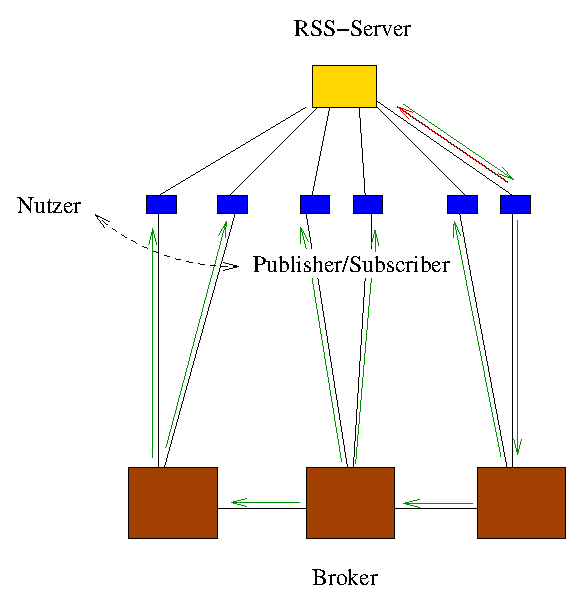
\includegraphics[bb=-100 0 200 250,scale=0.6]{RSSPubSub}
\end{frame}

\begin{frame}
  \frametitle{Ansatz: Ein Publisher}
  \begin{itemize}
  \item Ein Publisher w�rde ausreichen, um Feed herunterzuladen
  \item Alle weiteren Nutzer  bzw. Subscriber w�rden den Feed �bers Netzwerk erhalten
  \end{itemize}
  
  \pause
  Vorteil:\\
  Wenige Anfragen an den RSS-Server
  \vspace{0.5cm}
  
  \pause
  Problem:\\
  Aktualit�t der Feeds!\\
  $\longrightarrow$ lange �bertragungszeiten in Abh�ngigkeit von Netzstruktur\\
  u. U. aufw�ndiger Auswahlprozess\\
  Single Point of Failure
\end{frame}

\begin{frame}
  \frametitle{Aktualit�t vs. Server-Belastung}
  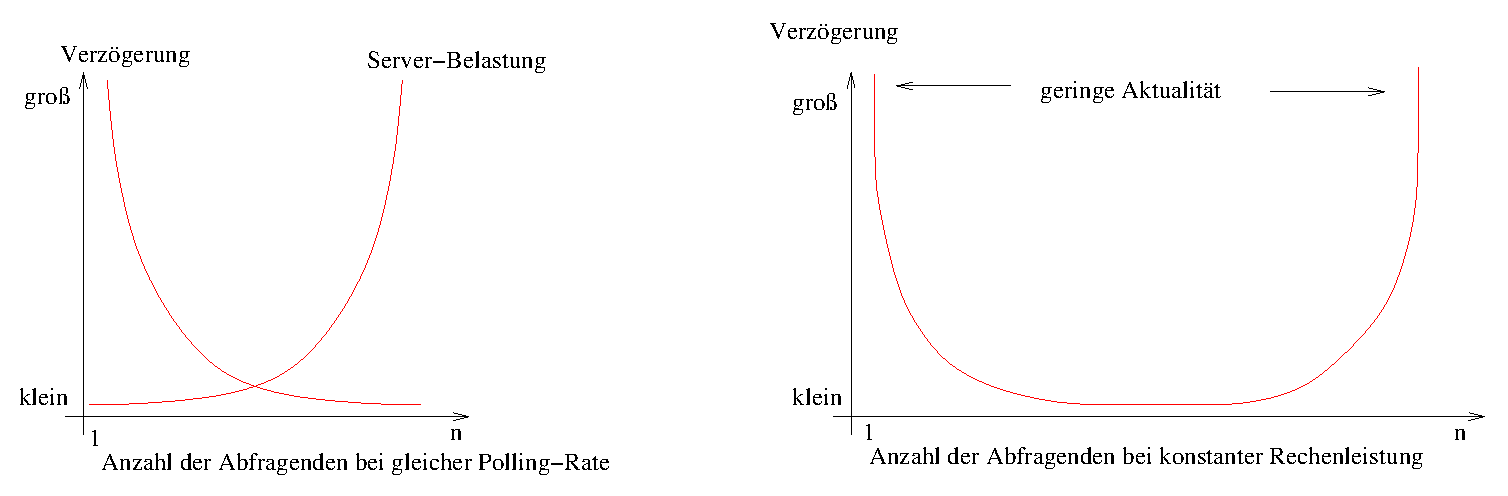
\includegraphics[bb=40 0 200 250,scale=0.5]{Verzoegerung}
\end{frame}

\begin{frame}
  \frametitle{Ansatz: Mehrere Publisher}
  \begin{itemize}
  \item Mehrere Publisher laden Feed herunter
  \item $\rightarrow$ Mindestens so viele, dass gewisse Aktualit�t der Feeds erreicht wird
  \item $\rightarrow$ H�chstens so viele, dass Server nicht �berlastet wird
  \end{itemize}
  \vspace{0.5cm}
  
  $\longrightarrow$ Ein optimaler Kompromiss soll erreicht werden
  
\end{frame}

\begin{frame}
  \frametitle{Frage:}
  Wie k�nnen sich die Publisher dar�ber abstimmen, wer als n�chstes den aktuellen Feed abholt?
\end{frame}

\begin{frame}
  \frametitle{Herausforderungen}
  Entwicklung eines bzw. mehrerer Algorithmen zur \dots
  \begin{itemize}
  \item \dots Koordinierung der Publisher
  \item \dots Ermittlung der RSS-Server-Auslastung
  \end{itemize}
\end{frame}

\begin{frame}
  \frametitle{Erwartungen an den Algorithmus}
  Der Entwurf des Algorithmus sollte unter folgenden Gesichtspunkten erfolgen:
  \begin{itemize}
  \item Vermeidung von \glqq Hotspots\grqq
  \item Broker sollen Parameter automatisch einstellen bzw. beziehen
  \item Parameter sollen sich den dynamischen Gegebenheiten des Netzes anpassen
  \item Netz soll auftretende Fehler �berstehen und selbst�ndig beseitigen
  \end{itemize}
\end{frame}

\begin{frame}
  \frametitle{Vorteile des Ansatzes}
  Vorteile gegen�ber �hnlichen Ans�tzen (wie z.B. FeedTree\cite{SandlerEtAl:2005:FeedTree}):
  \begin{itemize}
  \item L�sung kann sich problemlos in bestehende RSS-Architektur integrieren
  \item Bestehende Client-Software kann weiter verwendet werden
  \item Komplette Neukonstruktion eines Pub/Sub-Systems ist nicht notwendig\\
    $\longrightarrow$ in REBECA\cite{MuFiBu:2001:ArchFrameECommApp} sind Filtertechniken bereits integriert
  \end{itemize}
\end{frame}

\subsection*{Koordinierung der Publisher}

\begin{frame}
  \frametitle{Koordinierung der Publisher}
  \begin{itemize}
  \item Jeder Publisher w�hlt zuf�lligen Zeitpunkt innerhalb eines zeitlichen Intervalls, um n�chsten Feed herunterzuladen
  \item Erh�lt er neuen Feed �ber das Notifikationssystem, wird neuer Zeitpunkt gew�hlt
  \end{itemize}
  \frametitle{Wahl eines zuf�lligen Zeitpunktes}
  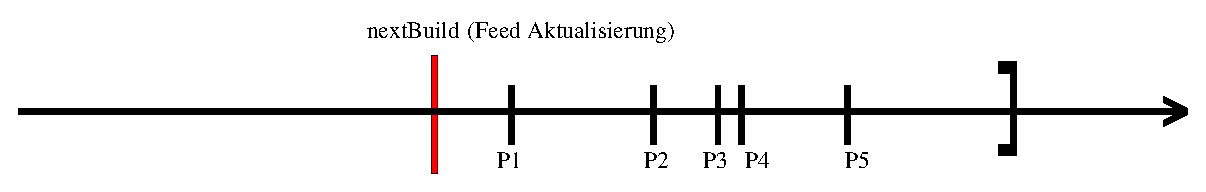
\includegraphics[bb=-40 0 200 150,scale=0.5]{Platzierungen}
\end{frame}

\section{Ergebnisse}

\begin{frame}
\frametitle{Anpassung der Polling-Perioden}
  \includepng{Referenzverlauf.png}
\end{frame}

\begin{frame}
\frametitle{Keine Ausbalancierung}
  \includepng{NoBalancing.png}
\end{frame}

\section{Literatur}
\begin{frame}[allowframebreaks]
  \bibliography{../bibdatabase}
\end{frame}

\end{document}
